\section{Thiết kế cơ sở hạ tầng trên nền tảng AWS}

Môi trường thực nghiệm được thiết kế và triển khai trên nền tảng Amazon Web Services (AWS) nhằm đảm bảo tính linh hoạt, khả năng mở rộng tự động và mức độ sẵn sàng cao (High Availability). Kiến trúc hệ thống phân bổ dịch vụ trên nhiều Vùng khả dụng (Availability Zones - AZs) trong cùng một VPC (Virtual Private Cloud) để triệt tiêu các điểm lỗi đơn lẻ (SPoF) và tối ưu hóa khả năng chịu lỗi vật lý.

Chi tiết mô hình kiến trúc hạ tầng AWS được minh họa cụ thể trong Hình \ref{fig:aws-infra-architecture}.

\begin{figure}[htbp]
    \centering
    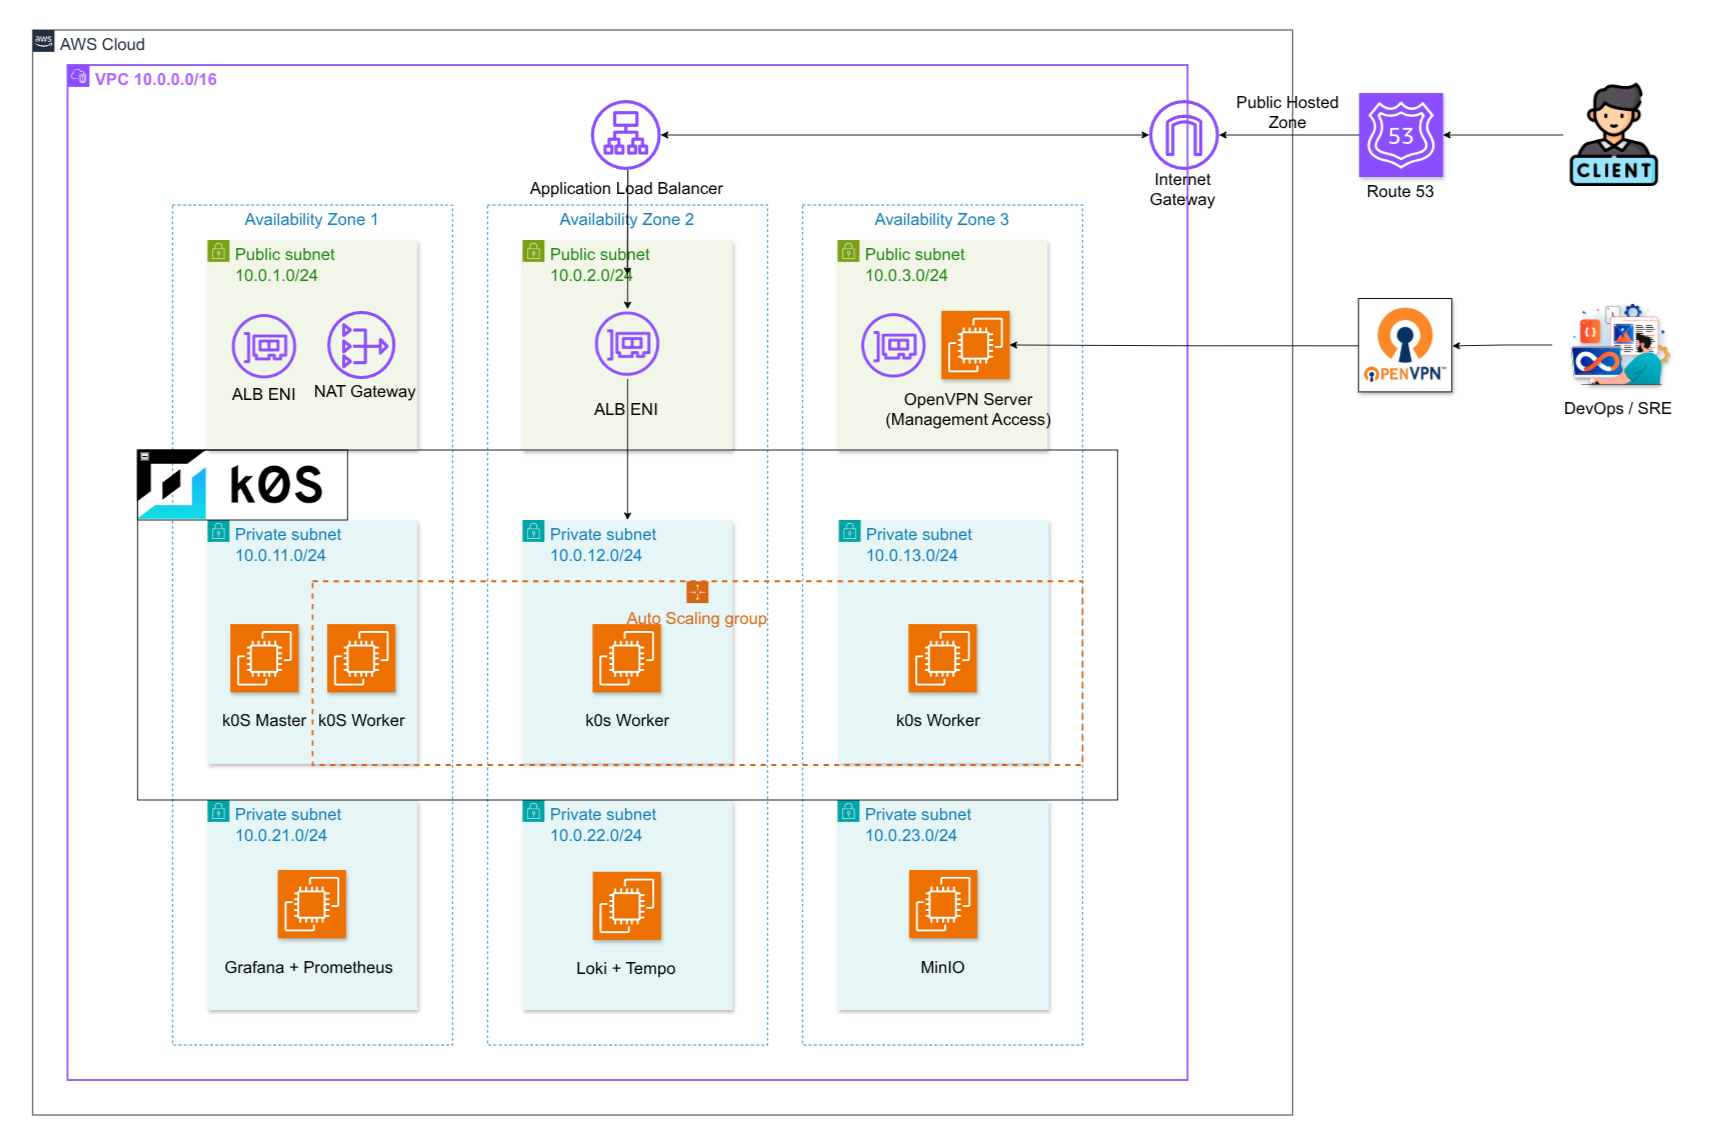
\includegraphics[width=0.8\textwidth]{graphics/chapter-5/cloud.png}
    \caption{Kiến trúc triển khai cơ sở hạ tầng trên nền tảng AWS}
    \label{fig:aws-infra-architecture}
\end{figure}

Kiến trúc hạ tầng bao gồm ba lớp chức năng chính:
\begin{itemize}
    \item \textbf{Lớp mạng (Networking Layer):} VPC dải mạng \texttt{10.0.0.0/16} được chia làm các Public/Private Subnet trên 03 AZs (us-east-1a, us-east-1b, us-east-1c). Lớp này sử dụng Internet Gateway (IGW) cho kết nối ngoài, NAT Gateway bảo mật cho phân vùng nội bộ, và Application Load Balancer (ALB) điều phối lưu lượng.
    \item \textbf{Lớp tính toán (Compute Layer):} Cụm Kubernetes được phân bổ trên cả 03 AZs để vận hành workloads. Trong đó, Master node đặt tại Private Subnet của AZ 1, các Worker node được phân tán ở các AZs khác nhau. Ngoài ra, hệ thống được bổ sung thêm Auto Scaling Group giúp hỗ trợ tăng giảm số máy Worker phục vụ lượng tải linh hoạt từ người dùng.
    \item \textbf{Lớp giám sát và quản trị (Management Layer):} Tích hợp Prometheus để thu thập dữ liệu huấn luyện (metrics) thời gian thực và Grafana để trực quan hóa phục vụ phân tích. Hệ thống quản trị được bảo mật thông qua OpenVPN Server đặt tại Public Subnet của AZ 3.
\end{itemize}

Để tối ưu hóa luồng lưu lượng và đảm bảo tính cô lập an toàn, chúng tôi thực hiện phân hoạch địa chỉ IP chi tiết cho toàn bộ các phân vùng mạng (Subnets) trong hệ thống như được trình bày trong Bảng \ref{tab:subnet-ip-allocation}.

\begin{center}
\captionof{table}{Phân hoạch địa chỉ IP cho các Subnets trong hệ thống thực nghiệm}
\label{tab:subnet-ip-allocation}
\footnotesize
\renewcommand{\arraystretch}{1.0}
\begin{tabular}{|C{3.2cm}|C{2.8cm}|C{3.0cm}|L{6.0cm}|}
\hline
\textbf{Vùng khả dụng (AZ)} & \textbf{Loại Subnet} & \textbf{Dải địa chỉ (CIDR)} & \textbf{Thành phần được triển khai} \\ \hline
\multirow{3}{*}{us-east-1a (AZ 1)} & Public & 10.0.1.0/24 & ALB ENI, NAT Gateway \\ \cline{2-4} 
 & Private (k0s) & 10.0.11.0/24 & k0s Master, k0s Worker Node \\ \cline{2-4} 
 & Private (Data) & 10.0.21.0/24 & Prometheus, Grafana \\ \hline
\multirow{3}{*}{us-east-1b (AZ 2)} & Public & 10.0.2.0/24 & ALB ENI \\ \cline{2-4} 
 & Private (k0s) & 10.0.12.0/24 & k0s Worker Node (Auto Scaling) \\ \cline{2-4} 
 & Private (Data) & 10.0.22.0/24 & Phân vùng dự phòng (Unused) \\ \hline
\multirow{3}{*}{us-east-1c (AZ 3)} & Public & 10.0.3.0/24 & OpenVPN Access Server \\ \cline{2-4} 
 & Private (k0s) & 10.0.13.0/24 & k0s Worker Node \\ \cline{2-4} 
 & Private (Data) & 10.0.23.0/24 & Phân vùng dự phòng (Unused) \\ \hline
\end{tabular}
\end{center}

Cơ sở hạ tầng mạng và tính toán này thiết lập một môi trường thực nghiệm có tính chân thực cao, tương đương với các hệ thống Cloud Production. Đây là nền tảng cốt lõi để thực hiện các kịch bản kích hoạt sự cố nhân tạo (Chaos Injection) liên quan đến \textit{Pod failure} và \textit{Node failure}, từ đó đo lường chính xác thời gian phục hồi và độ ổn định của giải pháp đề xuất so với cơ chế mặc định của Kubernetes.

\section{Triển khai cơ sở hạ tầng sử dụng Terraform}

Để đảm bảo tính tự động hóa, tính nhất quán và khả năng tái lập nhanh chóng cho môi trường thực nghiệm, toàn bộ tài nguyên hạ tầng trên AWS được định nghĩa và khởi tạo dưới dạng mã nguồn (Infrastructure as Code - IaC) thông qua công cụ Terraform. Việc này giúp triệt tiêu các sai sót cấu hình thủ công và kiểm soát chặt chẽ trạng thái tài nguyên thông qua tệp tin \texttt{terraform.tfstate}.


Quy trình áp dụng hạ tầng được thực hiện qua các lệnh tiêu chuẩn của Terraform bao gồm: \texttt{terraform init} (khởi tạo môi trường), \texttt{terraform plan} (kiểm tra dự báo thay đổi) và \texttt{terraform apply} (thực thi khởi tạo thực tế trên AWS). 


\section{Cấu hình các công cụ sử dụng Ansible}

Để tự động hóa cấu hình hệ điều hành và thiết lập phần mềm trên các máy chủ EC2 đã được khởi tạo bởi Terraform, chúng tôi sử dụng công cụ Ansible. Với kiến trúc không tác nhân (\textit{agentless}), Ansible thực hiện truyền tải các cấu hình thông qua kết nối SSH bảo mật, giúp thiết lập môi trường đồng bộ, nhất quán và giảm thiểu tối đa các thao tác quản trị thủ công. Các chỉ thị cấu hình được khai báo dưới dạng tệp tin YAML (\textit{Ansible Playbooks}).

\subsection{Cấu hình dịch vụ mạng riêng ảo sử dụng OpenVPN}

Dịch vụ OpenVPN Server được cấu hình và thiết lập tự động thông qua Ansible trên máy chủ đặt tại Public Subnet của AZ 3. Vai trò của thành phần này là thiết lập một đường truyền mã hóa bảo mật từ xa (VPN Tunnel) cho phép quản trị viên truy cập an toàn vào dải mạng nội bộ (Private Subnet) của VPC để thực hiện các thao tác quản trị cụm Kubernetes và hệ thống giám sát mà không cần công khai các cổng dịch vụ ra Internet.

\subsection{Cấu hình cụm Kubernetes}

Quy trình thiết lập cụm Kubernetes được tự động hóa hoàn toàn bằng Ansible Playbook bao gồm các công đoạn chính:
\begin{itemize}
    \item \textbf{Chuẩn bị môi trường:} Tắt phân vùng swap, cấu hình các tham số nhân hệ điều hành (\textit{sysctl}) cho mạng container và cài đặt container runtime (như \texttt{containerd}).
    \item \textbf{Cấu hình Master Node:} Khởi tạo nút điều khiển (Control Plane), thiết lập tệp cấu hình \texttt{kubeconfig} và cài đặt Container Network Interface (CNI) để thiết lập mạng nội bộ cho các Pods.
    \item \textbf{Gia nhập các Worker Nodes:} Ansible tự động trích xuất mã thông báo gia nhập (\textit{join token}) từ Master Node và thực thi lệnh kết nối các Worker Nodes phân tán trên các AZs vào cụm.
\end{itemize}

\subsection{Cấu hình hệ thống giám sát sử dụng Prometheus và Grafana}

Hệ thống giám sát được cấu hình tập trung trên máy chủ chuyên dụng đặt tại Private Subnet của AZ 1 nhằm đảm bảo tính toàn vẹn dữ liệu:
\begin{itemize}
    \item \textbf{Prometheus:} Được cấu hình thông qua Ansible để tự động phát hiện dịch vụ (\textit{service discovery}) trong cụm Kubernetes, thu thập dữ liệu metrics từ \texttt{node-exporter} (được Ansible cài đặt trên từng node) và \texttt{kube-state-metrics} theo chu kỳ 15 giây.
    \item \textbf{Grafana:} Được cấu hình sẵn các nguồn dữ liệu (\textit{Data Sources}) kết nối trực tiếp tới Prometheus và tự động nạp các bảng giao diện trực quan hóa (\textit{Dashboards}) để theo dõi hiệu năng tài nguyên hệ thống (CPU, RAM, Network) theo thời gian thực.
\end{itemize}
